\Introduction
\section{Скопления галактик}
В 2019 году произошел запуск космической обсерватории СРГ (Спектр-Рентген-Гамма) с телескопами 
eROSITA и ART-XC на борту. Основной задачей этих телескопов является создание обзора всего неба в 
рентгеновском диапазоне. Данные, полученные от этих телескопов будут использоваться для обнаружения 
астрономических объектов трёх категорий:

\begin{enumerate}
    \item Скопления галактик.
    \item Сверхмассивные чёрные дыры.
    \item Рентгеновские звёзды в галактике Млечный путь. 
\end{enumerate}

\subsection{Причины для изучения скоплений}

Наибольший интерес представляют скопления галактик. Скопления --- это гравитационно связанные 
системы, которые являются самыми большими динамически связанными структурами во Вселенной. 
Скопления галактик играют важную роль в задачах определения космологических параметров Вселенной.\\

Одной из главных задач космологии является построение карты скоплений галактик для того, чтобы 
можно было изучать их в совокупности. Для изучения скопления нужно знать его массу и красное 
смещение. Красное смещение - параметр, который позволяет узнать, на какое расстояние отдалился 
объект от наблюдателя за время измерения. Этот параметр является аналогом расстояния для отдалённых 
объектов. \\

Скопления по большей части состоят из тёмной материи, поэтому её изучение также зависит от 
имеющейся информации о скоплениях.
Когда мы наблюдаем за очень дальним скоплением, мы по факту получаем 
информацию из далёкого прошлого, так как время, за которое излучение от дальних объектов доходит до 
нас, может быть очень большим. Так можно изучать разные временные промежутки в развитии Вселенной.
Кроме того, соотношение компонент материи в 
скоплениях должно отражать средний состав Вселенной, что позволяет измерить вклад барионов в общую
плотность Вселенной.\\

\subsection{Данные телескопов в различных спектральных диапазонах}

Скопления галактик можно обнаружить исследуя данные различных диапазонов.\\

В первую очередь стоит упомянуть рентгеновский диапазон. Скопления выдают себя в рентгеновском 
диапазоне из-за присутствия в их составе горячего газа, излучающего энергию в рентгеновском 
диапазоне. Этот диапазон считается самым подходящим для поиска скоплений, так как их излучение 
в рентгеновском диапазоне имеет более точную корелляцию с массой скоплений (чем у других диапазонов), 
что позволяет более детально изучать эти объекты. Полные обзоры неба, полученные рентгеновским 
телескопом eROSITA, появятся к июню 2020 года, поэтому на данный момент есть возможность 
подготовить модели для сегментации данных на примере других диапазонов.\\

Также важным диапазоном для изучения скоплений является микроволновый диапазон. В этой области данных 
скопления галактик проявляются из-за того, что существует реликтовое излучение, которое заполняет 
собой всю Вселенную. Из-за своего состава скопления искажают это излучение, и по этим искажениям 
их можно наблюдать.\\ 

Поскольку скопления галактик состоят из галактик, которые сами по себе излучают энергию в видимом 
диапазоне, вполне логично для поиска скоплений использовать и оптические телескопы. Однако здесь 
препятствием может послужить тот факт, что скопления наблюдаются не как цельные структуры, а как 
совокупности нескольких галактик. \\

Данных в рентгеновском диапазоне сейчас не доступны, исследования для микроволнового диапазона уже 
существуют (будут упомянуты в обзоре существующих решений). Оптические данные находятся в общем 
доступе и есть возможность исследовать именно их, и впоследствии перейти к анализу совокупности 
данных из разных диапазонов.\\

\begin{figure}[h]
    \center{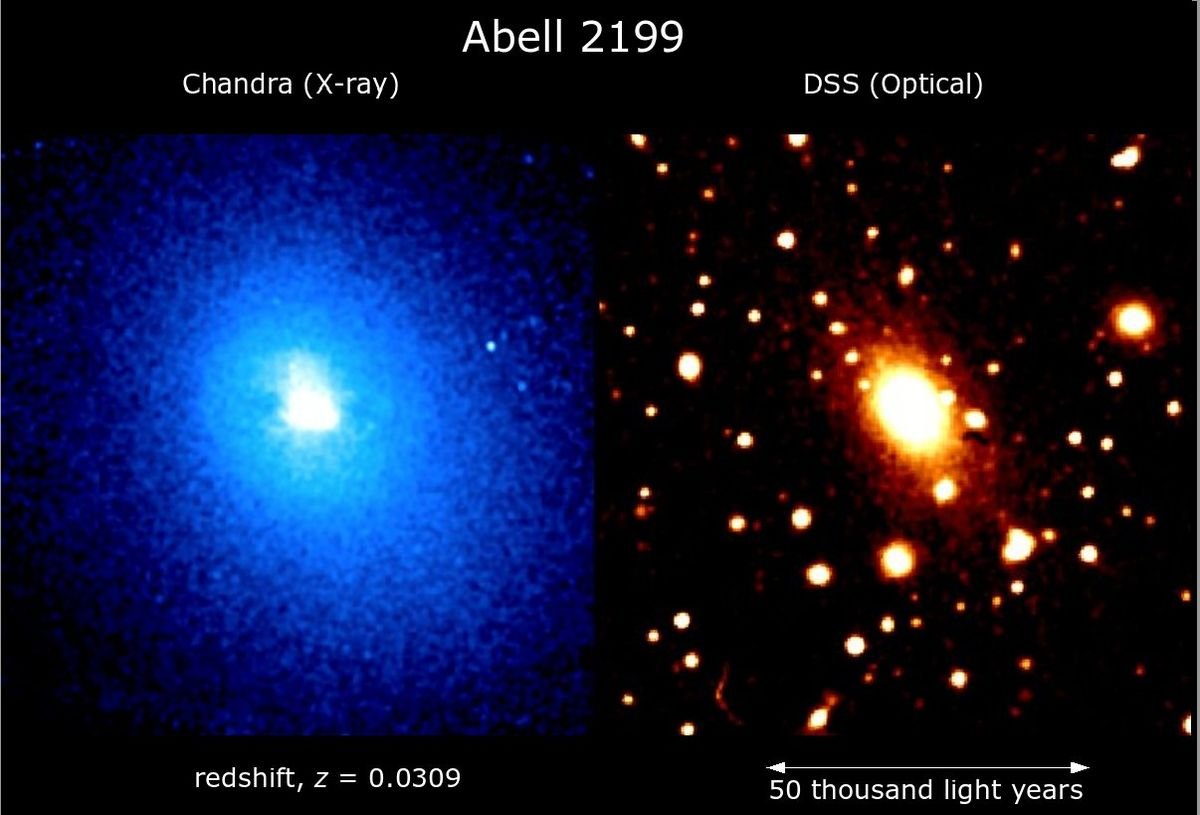
\includegraphics[width=0.7\linewidth]{comparison0}}
    \caption{Скопление <<Абель 2199>> в рентгеновском и оптическом диапазонах. \cite{Abell}}
\end{figure}


На текущий момент существует большое количество 
оптических телескопов, и, как следствие, большое количество данных, извлеченных с их помощью. В 
данной работе будут использоваться данные телескопа Pan-STARRS1, который является частью системы 
телескопов Pan-STARRS (Panoramic Survey Telescope and Rapid Response System). Обзор этого телескопа
покрывает самую большую область неба и покрывает те объекты, данные которых позднее будут получены 
телескопом eROSITA. Кроме того, его данные находятся в общем доступе \cite{Panstarrs}.\\

С появлением новых телескопов с новыми возможностями и характеристиками параллельно развиваются и 
методы обработки их данных. Чаще всего алгоритмы создаются под конкретный телескоп и под конкретный 
диапазон, и для более современных телескопов с более чувствительными датчиками они просто не подойдут.
Характеристики телескопа eROSITA позволят получить рентгеновские данные 
очень высокого качества (то есть с низким количеством шума), на них можно будет детектировать новые
скопления максимально точно. Поэтому есть возможность применить новые алгоритмы на таких данных.\\


\section{Нейросетевые методы}
В последние годы методы глубокого обучения стали играть важную роль в анализе данных. Нейросетевые 
модели показывают высокие результаты в области компьютерного зрения и в частности в задачах 
сегментации и детекции. Всё более часто они применяются и для решения задач астрофизики. Методы 
глубокого обучения дают много преимуществ при анализе космических данных: 

\begin{enumerate}
    \item Стандартные алгоритмы сегментации усредняют информацию по нескольким каналам,
        в то время как с помощью нейросети можно охватить данные полностью и исследовать вопрос с 
        новой стороны. Таким образом, нейросеть будет получать <<сырые>> данные, что экономит время 
        и исключает необходимость контролировать процесс предобработки данных. 
        Кроме того, нейросеть, используя все данные, может получить информацию о 
        калибровке телескопа прямо из обзоров, что невозможно сделать при использовании классических 
        методов.
    \item Аналогичнные методы можно использовать для сегментации одновременно разнородных данных. 
        То есть для улучшения качества сегментации можно исследовать параллельно разные диапазоны 
        частот и находить взаимосвязь между разными спектрами.
    \item Каждый из классических методов имеет свои достоинства и недостатки, и для каждого 
        диапазона излучения существуют свои алгоритмы, в то время как 
        нейросеть может стать универсальным средством для сегментации.
\end{enumerate}

\section{Каталоги скоплений}
Для обучения нейросетевых моделей требуется иметь большое количество данных, детектированных другими
способами. Для таких целей будут использоваться существующие каталоги скоплений галактик:

\begin{enumerate}
	\item PSZ2. Этот каталог был получен по данным <<Планка>>  при помощи алгоритмов 
	согласованного мультифильтра и PowellSnakes.
	\item MCXC (Meta-Catalogue of X-ray detected Clusters). Это объединенный каталог из всех 
	других каталогов скоплений, полученных из данных телескопа ROSAT.
	\item RedMaPPer (Red-sequence Matched-filter Probabilistic Percolation). Каталог скоплений, 
	полученный с помощью одноимённого алгоритма из данных оптического диапазона.
\end{enumerate}


В более формальном и подробном виде задачу можно описать так: при имеющихся обработанных данных, 
полученных из космических обзоров, требуется получить матрицы сегментации, где для каждого пикселя 
матрицы мы будем иметь информацию о вероятности, с которой в данном пикселе находится скопление. 
Впоследствии координаты пикселей изображений можно преобразовать в небесные координаты способом, 
обратным к способу, с помощью которого были получены изображения космических обзоров. На полученных 
масках можно будет детектировать скопления. Главной целью является создание итогового каталога 
скоплений, найденных в разных диапазонах.\\

Пока что не существует какого-то универсального метода для сегментации и детекции скоплений 
на оптических данных, и есть возможность применить методы глубокого обучения в данной области.\\


